\documentclass{article}
\usepackage{import}
\subimport{../}{preamble}
\begin{document}

\section{Electronics Design}

\begin{figure}[bt]
\centering
{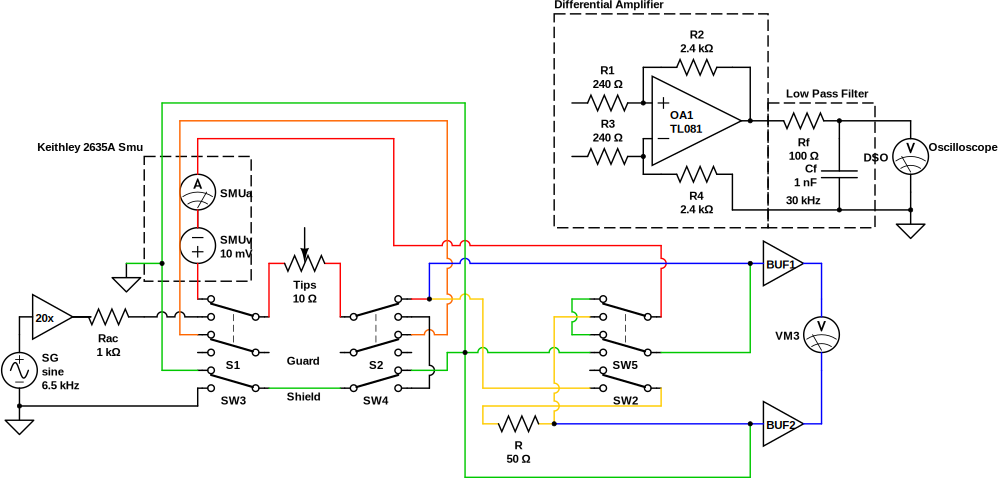
\includegraphics[width=15cm]{figures/tip_experiment_circuit_design}}
{\caption[Schematic of the electrical measurement circuit.]{\textbf{Schematic of the electrical measurement circuit.} The central routing box allows switching between a.c.\ and d.c.\ circuits and low-and high-bandwidth d.c.\ measurements. The a.c.\ circuit is used to align two AFM probes together while the d.c.\ circuit is used to measure spatially dependent signals from the gap between two AFM probes.}
\label{fig:circuit_design}}
\end{figure}

% Chamber electronics
The experiment chamber contains two triaxial connectors to send and return electronic signals through the chamber. These are wired to the Cu tip clamps to permit measurements of the electrical signal from the gap between the tips of two AFM probes. Control of electronics is done using a signal routing box to which the chamber triax cables are attached.
% Routing box
Electronics are split between the a.c.\ electronics that drive the resonant tip alignment procedure and the d.c.\ measurement electronics. The d.c.\ electronics are further split into a low and high bandwidth measurement circuit. The low bandwidth ($<\SI{10}{Hz}$) circuit measures electronics continually over long time periods, typically giving spatial information linked to sample separation. The high bandwidth circuit operates on a trigger to capture single shot events on much shorter time scales. The d.c.\ circuits are typically ran simultaneously while the a.c.\ and d.c.\ circuits are manually switchable. The schematic of this system is shown in \figurename~\ref{fig:circuit_design}.

% Circuit equipment
% A.c. circuit
The a.c.\ circuit consists of a simple signal generator connected to a $20\times$ voltage amplifier to drive the junction capacitance. This is used to resonantly drive an AFM cantilever into oscillation and align tips into a tip-to-tip dimer configuration. A \SI{200}{\ohm} current limiting resistor is placed after the amplifier to prevent damage to the tip junction in the event of a direct conductive contact.%
\footnote{The optimum resistance value is calculated using $R = V/I_{\mathrm{limit}}$ where $V=\SI{15}{V}$ typically and a safe current limit is $I_{\mathrm{limit}}=\SI{500}{\micro\ampere}$. This gives a resistance of \SI{30}{\kilo\ohm}.}
The circuit is then terminated at ground.
% D.c. circuit
The separate d.c.\ circuit consists of a source-meter unit (SMU, Keithley 2635A) used to apply a voltage across the junction and measure the current through the junction. The switchable high-bandwidth path routes the current through a $10^4\times$ gain transimpedance amplifier (Femto DLPCA-200) and then a further combined $10\times$ amplification/\SI{1}{MHz} low-pass filtering stage (SRS SR560). The amplified voltage is measured on a digital storage oscillation (DSO) with the shield forming the return path for the current back to the SMU via the routing box.

% Circuit separability to reduce noise
The fundamental feature of combined circuity is their separability. The a.c.\ circuit is not required to be low-noise but the d.c.\ circuitry is used to measure low-level currents. For the d.c.\ circuit to operate correctly it must be isolated from the other electronics. The a.c.\ circuit remains completely disconnected {\color{red} and grounded} when the d.c.\ circuit is in operation.
% Other considerations to reduce noise
In such an experiment where the aim is to measure small, sensitive currents, reducing the noise to a minimum is imperative. The noise floor at low bandwidths sets the minimum current which can be measured while the noise at high bandwidth (high frequencies) sets the conductance resolution and minimum trigger level for single shot measurements.
The reduced bandwidth of the SMU ($<\SI{10}{Hz}$) removes much of the noise from {\color{red}basic} measurements. Noise is reduced by using manual toggles switches over electrically controlled relays. All electronic chassis are grounded to a single point on the SMU to prevent EMI coupling and ground loops. Triax cabling is used with guarded connections running through the system except at the experiment chamber, which is grounded, to prevent leakage currents.

% Fast d.c. circuit
%The d.c. circuit functions to measure both the low bandwidth electronic response of a tip system as the gap size is reduced as well as the high bandwidth temporal response, triggered upon passing a specified threshold. To achieve this the low bandwidth measurement circuit must have a low impedance to best measure the gap conductance, modelled as a variable resistor. As a result, out of all possible circuit designs, a transimpedance amplifier is used to directly measure the current in series with the gap.

% Optimum circuit parameters
The operating standards and limitations of the high bandwidth measurement circuit are shown in Fig.~\ref{fig:hb_electronics_limits}. The value of the current limiting resistor, $R$, used to prevent overloading in the circuit is determined from these calculations using,
\begin{equation}
R = \frac{AV}{0.95V_{\mathrm{overload}}},
\end{equation}
where $V$ is the operating voltage of the measurement circuit, $A$ is the amplifier gain and$V_{\mathrm{overload}}$ is the minimum overload voltage for the circuit at a given voltage $V$ (determined by whichever limit is surpassed first, either the maximum input current of \SI{5}{mA}  pre-amplification or the maximum output voltage of \SI{5}{V})
\footnote{The relation between the current input into the amplifier and the amplifier output voltage is $V = AI$ hence $I_{\mathrm{limit}} = V_{\mathrm{overload}}/A$}.
The prefactor of 0.95 is used to prevent the current getting to the actual overload point. As it is assumed that we aim to work at \SI{10}{mV} (reasonable since we want good signal to noise with minimal electrostatic tip attraction and chance to overload the input/output current amplifier stages) a resistance of \SI{240}{\ohm} is used as it is close to the calculated value and provides some extra headroom for increasing the voltage.

\begin{figure}[h]
\centering
%\fcapside[\FBwidth]
{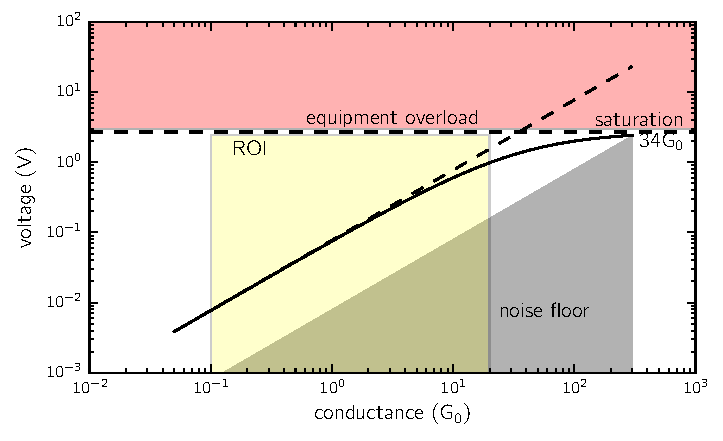
\includegraphics{figures/hb_electronics_limits}} % put voltage on right axis and current on left
{\caption[Characterisation of electronic measurements based on junction conductance.]{\textbf{Characterisation of electronic measurements based on junction conductance.} Solid lines show the calculated oscilloscope voltages for given junction conductances at selected voltages with use of current limiting resistor of $R=\SI{241}{\ohm}$ to prevent saturation. Dashed lines show the calculated oscilloscope voltages for the case without the current limiting resistor.}
\label{fig:hb_electronics_limits}}
\end{figure}

The overload/saturation characteristics come from the data sheets of the SRS SR570 current amplifier while the noise floor is measured. The minimum trigger level is determined as the point at which the measured voltage crosses the noise floor, below which the noise will incur false triggers.

\paragraph{Experimental Considerations}

For accurate electronic measurements using this circuit the series resistance is required to be measured to high precision. This is achieved using a SMU (Keithley 2635A).

Inverting this limiting resistance using $G = 1/R$ gives us a conductance limit to measurements. Conductances greater than this are small compared to the current limiting series resistance and are thus much harder to measure reliably. Ideally this value should be outside of the region of interest to prevent measurement error once the series resistance has been accounted for.

Current and transimpedance voltage measurements using the electronics circuit take the included series resistance into account using,
\begin{equation}
G_{\mathrm{junction}} = \left(G_{\mathrm{measured}}^{-1} - R_{\mathrm{series}}\right)^{-1}.
\end{equation}

\paragraph{Characterisation of the Electronics}

Conductance measurements are validated by...

\FloatBarrier
\end{document}